\documentclass{beamer}

\usepackage[utf8]{inputenc}

%% Title page formatting
\title{Tree cover variability increases from 2005 to 2100\\ in Sub-Saharan Africa}
\author{Eric Kalosa-Kenyon, Cody Carroll, Amy Kim}
\institute{University of California, Davis}
\date{}

\begin{document}

\frame{\titlepage}

\begin{frame}
    \frametitle{Introduction: climate system}
    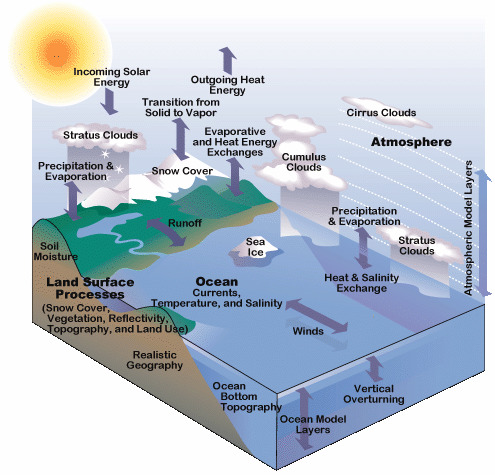
\includegraphics[height=3in]{../img/ccsm_diagram_picture.jpeg}

    https://www.ucar.edu/communications/CCSM/overview.html
\end{frame}

\begin{frame}
    \frametitle{Introduction: climate system modeling}
    \begin{itemize}
        \item Climate change is driven by anthropogenic carbon forcing
        \item IPCC has developed representative carbon forcing trajectories
        \item Computer simulations are run predicated on particular forcing
            pathways
        \item These simulations are realizations of gridded meteorological PDEs
    \end{itemize}
    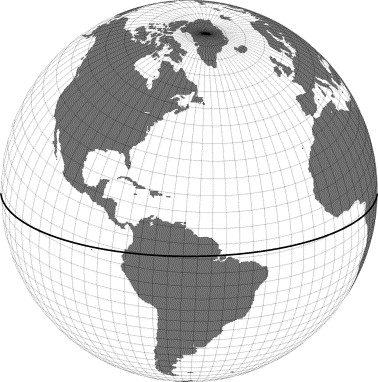
\includegraphics[width=\textwidth/2]{../img/greenland_pole_grid.jpg}
\end{frame}

\begin{frame}
    \frametitle{Introduction: climate system modeling}
    \begin{itemize}
        \item The Community Climate Model System has 5 components and a coupler:
            atmosphere, sea, land, sea ice, and land ice.
        \item We focus on the land system output from a single ensemble under
            the RCP4.5 experiment.

        \item $\theta\in\Theta, \{X_t|t\in\mathbb{Z}\} \textrm{ where }
            X_t\sim \textrm{ARMA}_\theta$
    \end{itemize}
\end{frame}

\begin{frame}
    \frametitle{Introduction: leaf area index (LAI)}
    \begin{columns}

        \column{2in}
            \begin{itemize}
                \item LAI is unitless quantity (leaf area ($m^2$))/(ground area ($m^2$))
                \item "Comparative Physiological Studies on the Growth of Field Crops" Watson 1947 Annals of Botany
                \item Bounded below by 0, above by physiological limits
                \item We interrogate a location in a tropical rainforest
            \end{itemize}

        \column{3in}
            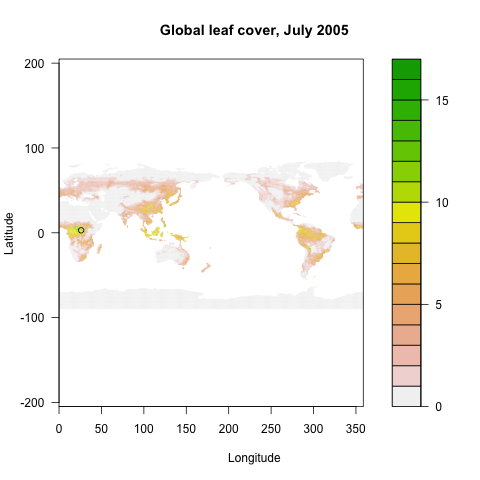
\includegraphics[height=3in]{../img/LAI_global_t0.png}

    \end{columns}
\end{frame}


\begin{frame}
    \frametitle{Raw data}
    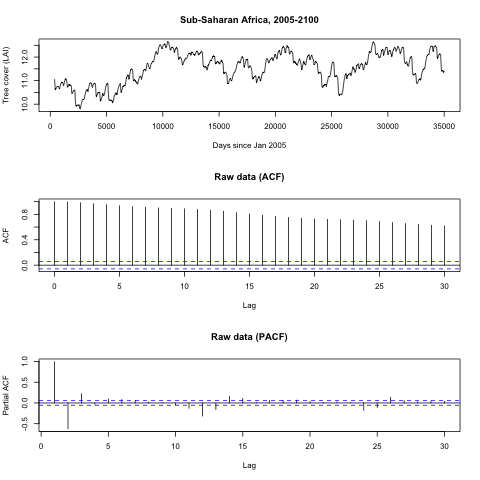
\includegraphics[height=3in]{../img/pacf_acf_raw.png}
\end{frame}

\begin{frame}
    \frametitle{Detrended data}
    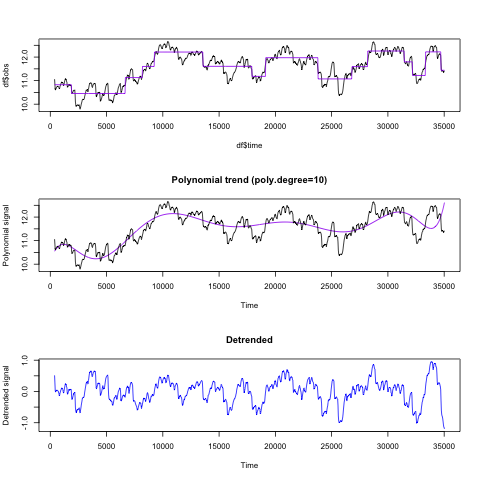
\includegraphics[height=3in]{../img/detrended_acf_pacf.png}
\end{frame}

\begin{frame}
    \frametitle{Standardize variance}
    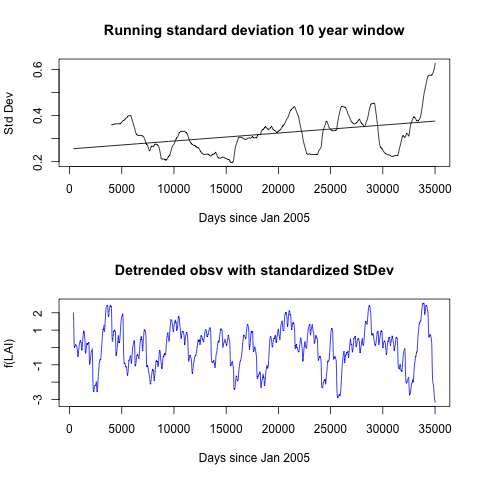
\includegraphics[height=3in]{../img/standatdized_var_LAI.png}
\end{frame}

\begin{frame}
    \frametitle{Standardized variance}
    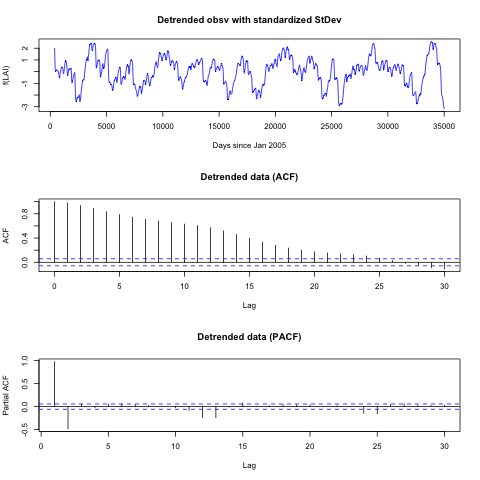
\includegraphics[height=3in]{../img/detrended_stdzd_acf_pacf.png}
\end{frame}

\end{document}
